\documentclass[tikz,border=7pt]{standalone}
\usepackage{libertinus}
\usepackage{amsmath}
\usetikzlibrary{
  arrows.meta,
  backgrounds,
  calc,
  decorations.markings,
  fit,
  positioning
}

\definecolor{accent}{RGB}{38,103,115}
\definecolor{softgray}{RGB}{244,245,246}
\definecolor{midgray}{RGB}{123,128,132}

\tikzset{
  >={Latex[length=2.2mm,width=1.5mm]},
  flow/.style={-Latex,semithick,draw=black!72},
  accent flow/.style={-Latex,semithick,draw=accent},
  box/.style={
    draw=black!68,
    fill=softgray,
    rounded corners=1.2pt,
    align=center,
    inner xsep=5pt,
    inner ysep=4pt
  },
  accent box/.style={
    draw=accent,
    fill=accent!8,
    rounded corners=1.2pt,
    align=center,
    inner xsep=5pt,
    inner ysep=4pt
  },
  point/.style={circle,draw=black!75,fill=white,inner sep=1.7pt},
  accent point/.style={circle,draw=accent,fill=accent!10,inner sep=1.7pt},
  tinylabel/.style={font=\scriptsize,align=center},
  smalllabel/.style={font=\small,align=center},
  panel/.style={draw=black!28,rounded corners=2pt,inner sep=6pt}
}


\newcommand{\seqnode}[4][]{%
  \node[box,minimum width=1.02cm,minimum height=.72cm,#1] (#2) at (#3) {#4};%
}

\begin{document}
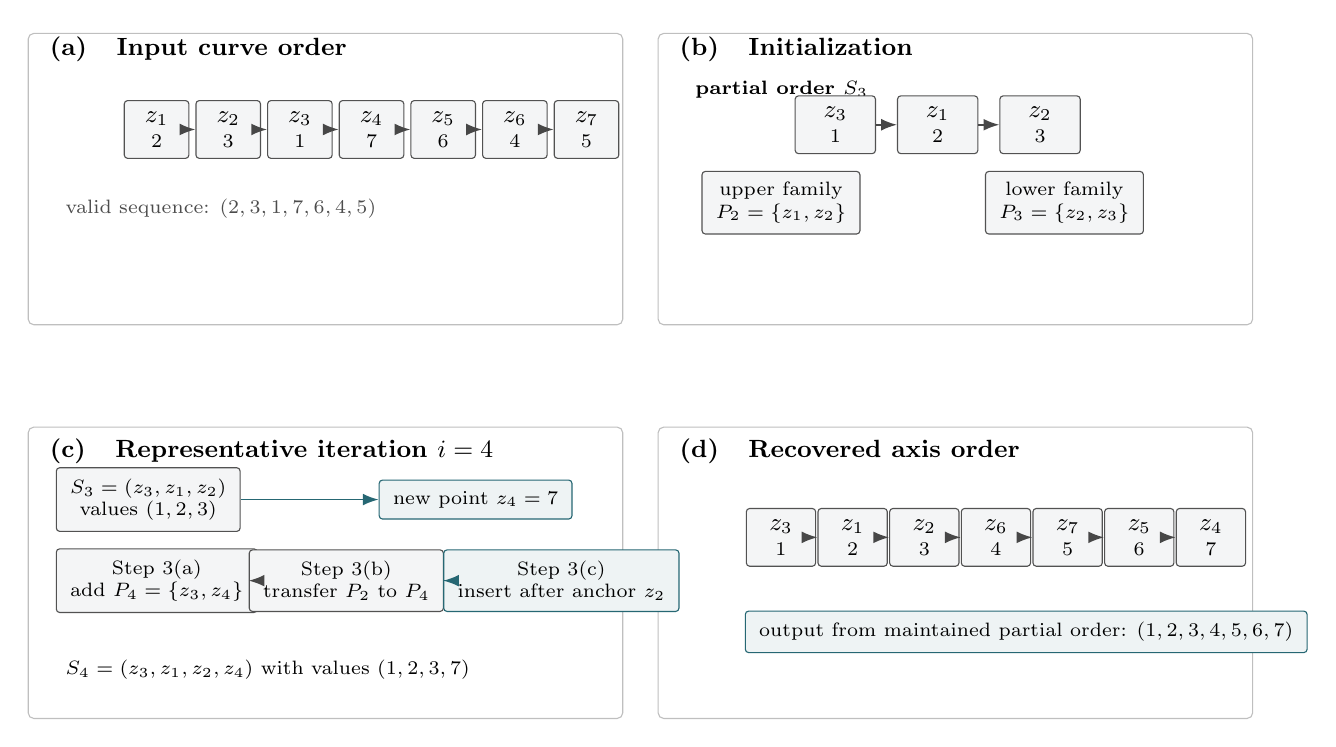
\begin{tikzpicture}[x=1cm,y=1cm,font=\small]
  % Panel anchors and borders.
  \coordinate (a0) at (0,5.1);
  \coordinate (b0) at (8.0,5.1);
  \coordinate (c0) at (0,0);
  \coordinate (d0) at (8.0,0);
  \foreach \o/\label/\title in {
    a0/(a)/Input curve order,
    b0/(b)/Initialization,
    c0/(c)/Representative iteration $i=4$,
    d0/(d)/Recovered axis order
  } {
    \node[anchor=north west,font=\small\bfseries] at ($ (\o)+(0.15,-0.12) $)
      {\label\quad \title};
  }

  % (a) Input.
  \foreach \value [count=\i] in {2,3,1,7,6,4,5} {
    \seqnode[minimum width=.82cm]{a\i}{$ (a0)+(0.72+0.91*\i,-1.42) $}{$z_{\i}$\\[-2pt]\scriptsize $\value$}
    \ifnum\i>1
      \draw[flow] (a\the\numexpr\i-1\relax.east) -- (a\i.west);
    \fi
  }
  \node[font=\scriptsize,text=black!70,anchor=west] at ($(a0)+(0.35,-2.42)$)
    {valid sequence: $(2,3,1,7,6,4,5)$};

  % (b) Initialization.
  \node[font=\scriptsize\bfseries,anchor=west] at ($(b0)+(0.35,-.92)$) {partial order $S_3$};
  \seqnode{b1}{$ (b0)+(2.25,-1.36) $}{$z_3$\\[-2pt]\scriptsize $1$}
  \seqnode{b2}{$ (b0)+(3.55,-1.36) $}{$z_1$\\[-2pt]\scriptsize $2$}
  \seqnode{b3}{$ (b0)+(4.85,-1.36) $}{$z_2$\\[-2pt]\scriptsize $3$}
  \draw[flow] (b1) -- (b2);
  \draw[flow] (b2) -- (b3);
  \node[box,font=\scriptsize,anchor=west] (up) at ($(b0)+(.55,-2.35)$)
    {upper family\\$P_2=\{z_1,z_2\}$};
  \node[box,font=\scriptsize,anchor=west] (lo) at ($(b0)+(4.15,-2.35)$)
    {lower family\\$P_3=\{z_2,z_3\}$};

  % (c) Representative step.
  \node[box,font=\scriptsize,anchor=west] (s3) at ($(c0)+(.35,-1.02)$)
    {$S_3=(z_3,z_1,z_2)$\\values $(1,2,3)$};
  \node[accent box,font=\scriptsize,anchor=west] (newp) at ($(c0)+(4.45,-1.02)$)
    {new point $z_4=7$};
  \draw[accent flow] (s3) -- (newp);

  \node[box,font=\scriptsize,anchor=west] (s3a) at ($(c0)+(.35,-2.05)$)
    {Step 3(a)\\add $P_4=\{z_3,z_4\}$};
  \node[box,font=\scriptsize,anchor=west] (s3b) at ($(c0)+(2.80,-2.05)$)
    {Step 3(b)\\transfer $P_2$ to $P_4$};
  \node[accent box,font=\scriptsize,anchor=west] (s3c) at ($(c0)+(5.27,-2.05)$)
    {Step 3(c)\\insert after anchor $z_2$};
  \draw[flow] (s3a) -- (s3b);
  \draw[accent flow] (s3b) -- (s3c);
  \node[font=\scriptsize,anchor=west] at ($(c0)+(.35,-3.18)$)
    {$S_4=(z_3,z_1,z_2,z_4)$ with values $(1,2,3,7)$};

  % (d) Final order.
  \foreach \label/\value [count=\i] in {z_3/1,z_1/2,z_2/3,z_6/4,z_7/5,z_5/6,z_4/7} {
    \seqnode[minimum width=.88cm]{d\i}{$ (d0)+(0.65+0.91*\i,-1.50) $}{$\label$\\[-2pt]\scriptsize $\value$}
    \ifnum\i>1
      \draw[flow] (d\the\numexpr\i-1\relax.east) -- (d\i.west);
    \fi
  }
  \node[accent box,font=\scriptsize,anchor=west] at ($(d0)+(1.1,-2.70)$)
    {output from maintained partial order: $(1,2,3,4,5,6,7)$};

  % Panel frames in the background.
  \begin{scope}[on background layer]
    \foreach \x/\y in {0/1.2,8/1.2,0/-3.8,8/-3.8} {
      \draw[black!25,rounded corners=2pt] (\x,\y) rectangle ++(7.55,3.7);
    }
  \end{scope}
\end{tikzpicture}
\end{document}
